%# -*- coding: utf-8-unix -*-
%%==================================================

\chapter{查找与排序}
\label{chap13}

\begin{itemize}[noitemsep,topsep=0pt,parsep=0pt,partopsep=0pt]
	\item 知识点:讲解相关知识点。
	\item 题型:直接上真题。
\end{itemize}

\section{知识点和方法论}

\subsection{知识点}
\begin{itemize}[noitemsep,topsep=0pt,parsep=0pt,partopsep=0pt]
	\item 查找成功长度和查找失败长度
	\item 折半查找算法
	\item 折半查找树的绘制
	\item 各种排序知道整体的流程
	\item 快速排序的partation代码要记住,可能要考试。
\end{itemize}

\subsection{方法论}

\section{真题实战}

\subsection{2010年408}
已知一个长度为16的顺序表L,七元素按关键字有序排列,若采用折半查找发查找一个L中不存储在的元素,则关键字的比较次数最多是(  )\newline
解:\newline
折半查找失败最多次数是树的高度求树的高度得到$\left \lfloor log_2{n} \right \rfloor + 1$ 就可以得到树的高度。\newline


\subsection{王道简单题}
具有12个关键字的有序表中,对每个关键字的查找概率相同,折半查找查找成功的平均查找长度为(   ), 者半查找查找失败的平均查找长度为(  ).\newline
A. 37/12   B. 35/12 C. 39/13 D. 49/13 \newline
解:\newline
记住折半查找算法的开始位置是从0开始到len-1结束。一定要画出者半查找树\newline
算查找失败的次数只要算下面方括号的上面的结点的wpl,再处于元素的个数\newline
\begin{figure}[H]
	\centering  % 环境中的内容居中排版
	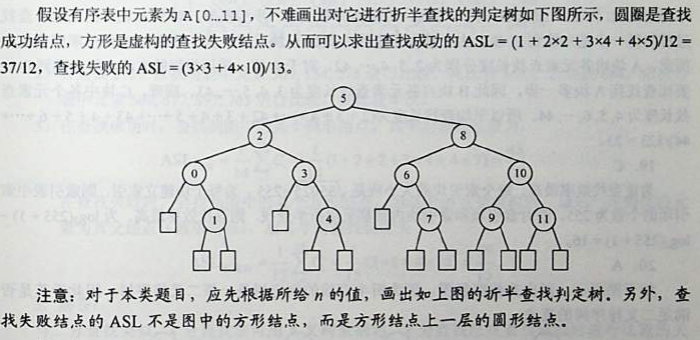
\includegraphics[scale=1]{example/chapter13/Annotation2019-09-25181550.png}
\end{figure}

\subsection{王道简单题考察希尔排序}
若数据元素序列{98, 36, -9, 0, 47,23, 1, 8, 10, 7}采用希尔排序系列序列是增量为4的一趟排序结果。\newline
解:\newline
\begin{figure}[H]
	\centering  % 环境中的内容居中排版
	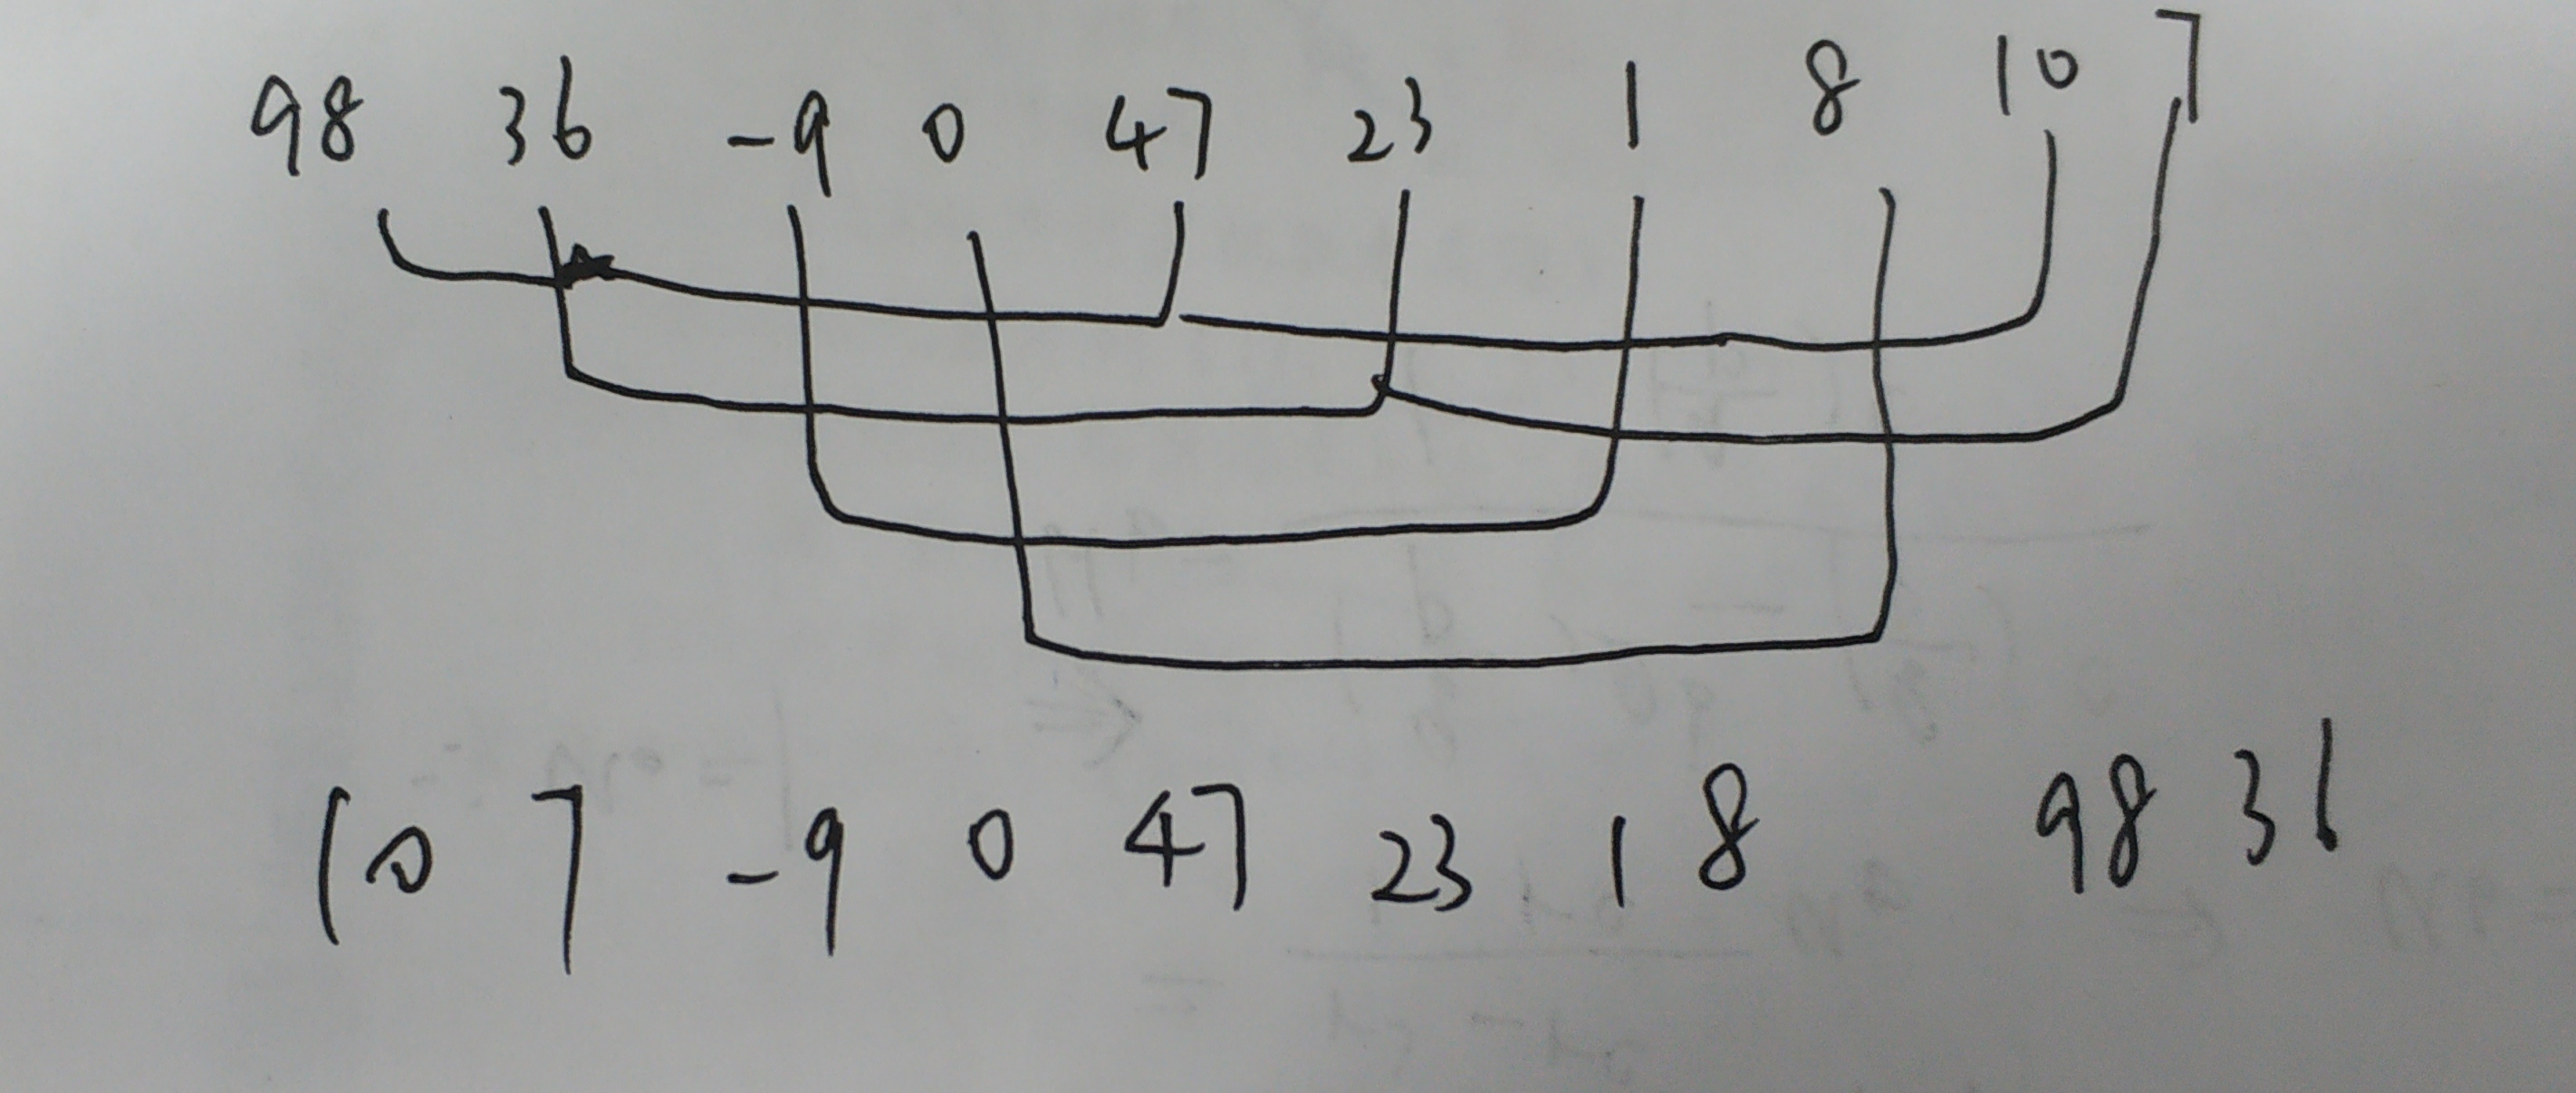
\includegraphics[scale=0.1]{example/chapter13/IMG_20190925_191655.jpg}
\end{figure}

\subsection{2015年408}
希尔排序的组内排序是()\newline
解:\newline
易知是直接插入排序。\newline

\subsection{2009年408}
若数据元素序列{11,12,13,7,8,9,23,4,5}是采用系列排序方法之一得到的第二趟排序后的结果,则该排序算法只能是(   )\newline
插入排序,因为局部有序,冒泡和选择都是有一些位置在他们最终的位置上。\newline













